\documentclass{beamer}
\usepackage{fontspec}
\usepackage{xunicode}
\usepackage{xltxtra}
\usepackage{xecyr}
\usepackage{hyperref}
\setmainfont[Mapping=tex-text]{DejaVu Serif}
\setsansfont[Mapping=tex-text]{DejaVu Sans}
\setmonofont[Mapping=tex-text]{DejaVu Sans Mono}
\usepackage{polyglossia}
\setdefaultlanguage{russian}
\setotherlanguage{english}
\usepackage{graphicx}
\usepackage{listings}
\lstdefinestyle{mycode}{
  belowcaptionskip=1\baselineskip,
  breaklines=true,
  xleftmargin=\parindent,
  showstringspaces=false,
  basicstyle=\footnotesize\ttfamily,
  keywordstyle=\bfseries,
  commentstyle=\itshape\color{gray!40!black},
  stringstyle=\color{red},
  numbers=left,
  numbersep=5pt,
  numberstyle=\tiny\color{gray},
}
\lstset{escapechar=@,style=mycode}
\usepackage{tcolorbox}
\usepackage{lipsum}

\newcommand{\cimg}[2]{%
	\begin{center}%
		\ifthenelse{\equal{#2}{}}{%
			\includegraphics[width=0.75\linewidth]{#1}
		}{%
			\includegraphics[width=#2\linewidth]{#1}
		}%
	\end{center}%
}

\usetheme{Antibes}
\useoutertheme{infolines}

\title{Curse Words Detector}
\subtitle{project}
\author{Беляев Станислав, Пластинин Виталий}
\institute{СПб АУ РАН}
\date{Весна 2016}

\setbeamercovered{highly dynamic}
\newcounter{saveenumi}
\newcommand{\seti}{\setcounter{saveenumi}{\value{enumi}}}
\newcommand{\conti}{\setcounter{enumi}{\value{saveenumi}}}

\begin{document}

\frame{\titlepage}

\section{Цели и задачи}
\begin{frame}[<+->]{Цели и задачи}
    \begin{enumerate}
        \item Модуль на питоне для блокировки слов
        \item Тесты
        \item Профиллирование работы
        \item Реализовать в виде NodeJS библиотеки
    \end{enumerate}
\end{frame}

\section{Данные}
\begin{frame}{Данные}
    \begin{tcolorbox}[colback=blue!5,colframe=blue!40!black,title=Реальный пример текста]
        всем пака с вами был данил 92 жди 12 части
        рости шамбарова да жалуйся в групе я тебя не баюсь да пашол ты в ростик шамбарова
        я тебя не баюсь я не буду руский учит зазазазазазазазаз
        ростик шамбарова меня не жэляют это тебя жэлеют тваи видео
    \end{tcolorbox}
    \begin{itemize}
        \item Простая лексика, много ошибок
        \item Порядка $94\%$ слов - среди первых $5000$ в частотном списке
        \item Много имен собственных, неологизмов
    \end{itemize}
\end{frame}

\section{Вероятностная модель замены слов}
\begin{frame}[t]{Вероятностная модель замены слов}
    Дано слово $w$, нужно найти ближайшее к нему "плохое" $c$
    $$argmax_c ~ {P(c|w)} = argmax_c ~ \left[ {P(w|c) \frac{P(c)}{P(w)}} \right]$$
    \begin{enumerate}
        \item $P(c)$ - насколько вероятно, что $c$ присутствует в тексте
            \begin{itemize}
                \item частотные списки взял у opencorpora
            \end{itemize}
        \item $P(w)$ - константа
        \item $P(w|c)$ - вероятность того, что автор написал $w$, подразумевая $c$
            \begin{itemize}
                \item edit distance $\leqslant 2$
            \end{itemize}
        \item $argmax_c$ - максимум по всем $c$
    \end{enumerate}
\end{frame}

\section{Вероятностная модель замены слов}
\begin{frame}
    Как считать edit dist?
    \begin{itemize}
        \item Вероятность замены чуть больше вероятность пропустить или добавить лишнюю букву
        \item Вероятность замены парных, похоже слышащихся, пишущихся, частых ошибок больше
    \end{itemize}
    Нормальная форма:
    \begin{itemize}
        \item Анализатор приводящий в нормальную форму дает вероятность успеха
        \item Также есть предиктор для несловарных слов (в том числе и для слов с ошибками)
    \end{itemize}
\end{frame}

\section{Алгоритм}
\begin{frame}{Алгоритм}
    Алгоритм:
    \begin{itemize}
        \item Препосчет - edit dist 1 для всех матных и для первых нескольких тысяч из частотного списка (порядка 30 Mb)
        \item Вход - слово w
        \item Найдем все хорошие нормальные формы, среди них лучшее "хорошее" и "плохое"
        \item Иначе - считаем edit dist (от всех нормальных форма начиная с наиболее вероятной) и смотрим в предпосчитанные, опять выбирая лучшее
        \item Иначе - считаем edit dist от всех слов их пред. пункта и делаем тоже самое (сюда мы попадем не часто)
    \end{itemize}
\end{frame}

\section{Архитектура проекта}
\begin{frame}[t]{Архитектура проекта}
    Модули на python3:
    \begin{enumerate}
        \item Purifier - main
        \item Analizier - работа с нормальной формой + предиктор (pymorphy2, реализация внутри на $C$, поэтому быстро). Еще был вариант взять Mystem от Яндекса, но он оказался слишком долгим
        \item Heurister - эвристическая замена цифр и латинских букв на русские
        \item Statisticer $\&$ Tester - классы для сбора статистики и тестов
    \end{enumerate}
    Особенности:
    \begin{itemize}
        \item Для экономии памяти можно замень словарь с стандартного dict() на prefix tree, значительно улучшив память, но пожертвовав производительностью
    \end{itemize}
\end{frame}

\section{Результаты}
\begin{frame}[t]{Результаты}
    \begin{center}
        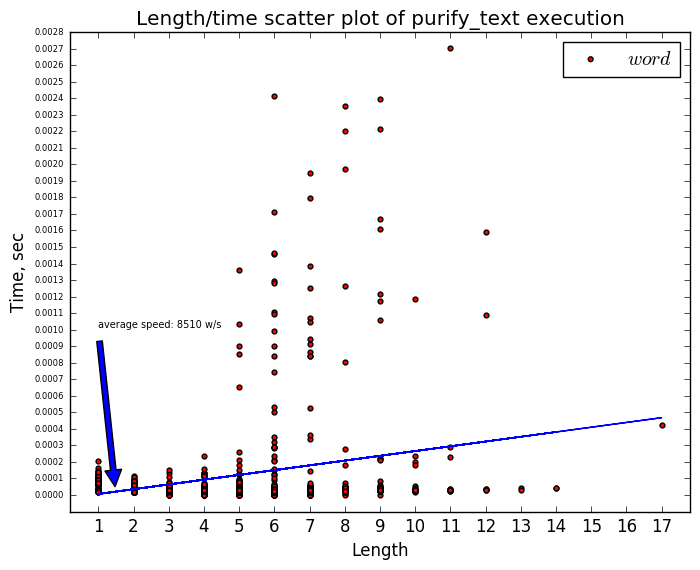
\includegraphics[width=0.70\linewidth]{../src/test/resources/plots/length_time_plot.png}
    \end{center}
\end{frame}
\begin{frame}
    Получилось:
    \begin{itemize}
        \item Довольно быстро работающий блокировщик (порядка $9000$ слов/сек.)
        \item Точность на реальных данных - $100 \%$ (на тех, что было)
        \item Поработать с профилировкой и оптимизацией на python
    \end{itemize}
    Не получилось:
    \begin{itemize}
        \item Библиотека для Node.js (время)
        \item Анализ с контекстом (частотные списки для пар слишком большие)
    \end{itemize}
\end{frame}

\section{Цели и задачи}
\begin{frame}[<+->]{Цели и задачи}
    \begin{enumerate}
        \item База слов
        \item Рассчёт ближайшего слова
        \item Замена слов
    \end{enumerate}
\end{frame}

\section{Архитектура проекта}
\begin{frame}[t]{Архитектура проекта}
\begin{enumerate}
	\item
	Собираем базу данных слов, так как текущие устарели
	\begin{enumerate}
	\item
	Обработали все слова на странице
	\item
	Все ссылки положили в очередь, взяли оттуда же следующую страницу
	\end{enumerate}
\item
    Дано плохое слово. Подбираем похожее хорошее.
        
\end{enumerate}
\end{frame}
\begin{frame}[t]{Архитектура проекта}
    Модули на python3:
    \begin{enumerate}
        \item Censor - работа со словами
        \item Crawler - обход сайтов
        \item DBHelper - для бд
    \end{enumerate}
\end{frame}

\section{Примеры}
\begin{frame}[t]{Примеры}
\begin{center}
\begin{enumerate}
	\item бл*дина -> льдина 
	\item ху*вничать -> чаёвничать
	\item раз*банный -> размётанный
	\item ж*пы -> окопы
\end{enumerate}
\end{center}
\end{frame}

\section{Конец}
\begin{frame}[t]{Конец}
    \begin{center}
    Спасибо за внимание
    \end{center}
	\begin{description}
		\item[GitHub:]  \url{github.com/StasBel/CurseWordsDetector}
		\item[GitHub:]  \url{github.com/vitalik239/ClilkBan}
	\end{description}
\end{frame}

\end{document}